\nolabel{section}{Приложение 1}

\section*{Запросы в Postman для проверки работы бэкенда}

\label{app:postman}

\begin{figure}[H]
	\centering
	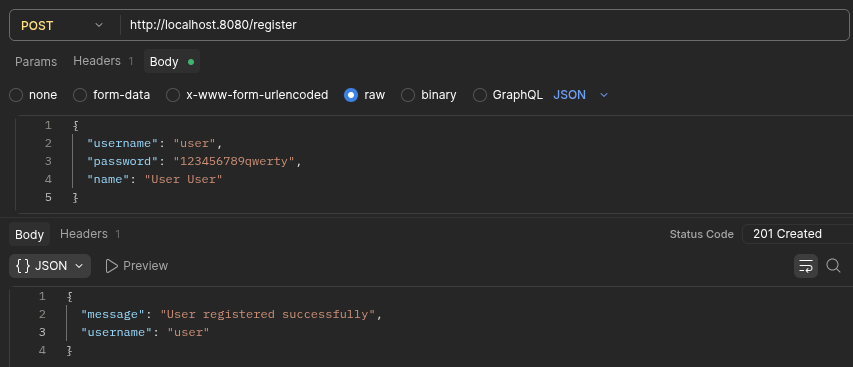
\includegraphics[width=1\textwidth]{images/postman/register.png}
	\caption{Запрос регистрации пользователя}
	\label{fig:register}
\end{figure}

\begin{figure}[H]
	\centering
	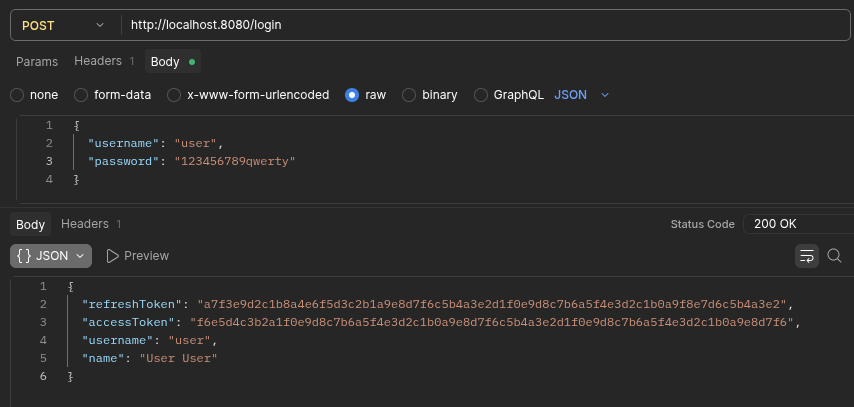
\includegraphics[width=1\textwidth]{images/postman/login.png}
	\caption{Запрос входа в систему}
	\label{fig:login}
\end{figure}

\begin{figure}[H]
	\centering
	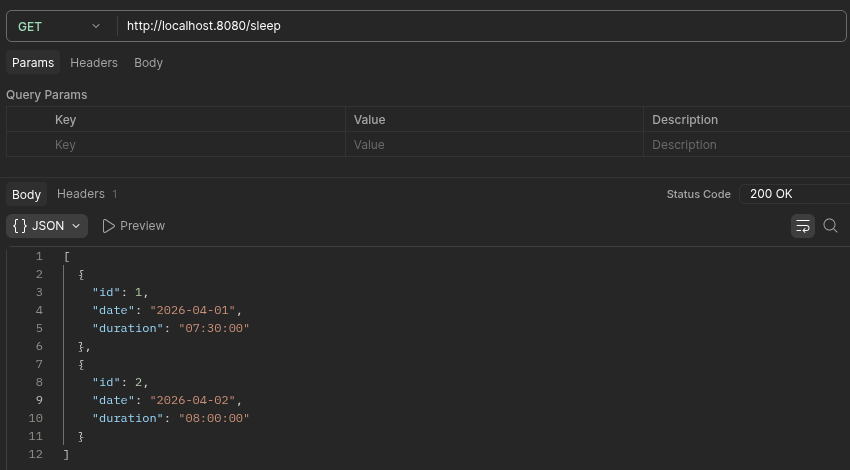
\includegraphics[width=1\textwidth]{images/postman/sleep_get.png}
	\caption{Запрос получения записей о сне}
	\label{fig:sleep_get}
\end{figure}

\begin{figure}[H]
	\centering
	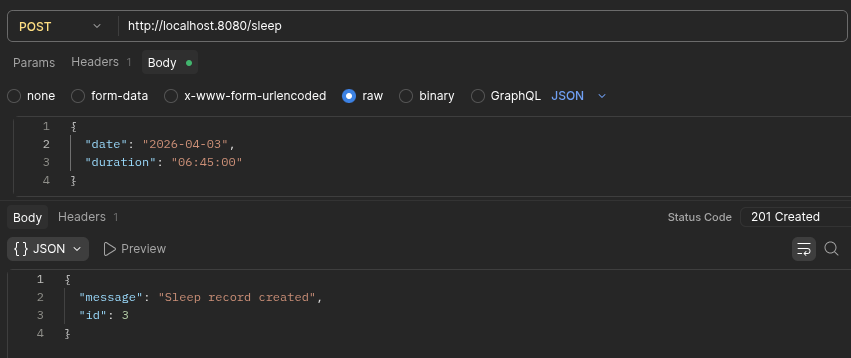
\includegraphics[width=1\textwidth]{images/postman/sleep_post.png}
	\caption{Запрос добавления записи о сне}
	\label{fig:sleep_post}
\end{figure}

\begin{figure}[H]
	\centering
	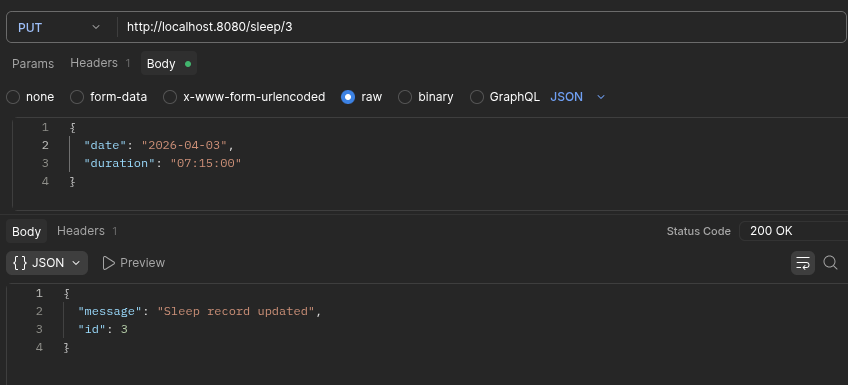
\includegraphics[width=1\textwidth]{images/postman/sleep_put.png}
	\caption{Запрос обновления записи о сне}
	\label{fig:sleep_put}
\end{figure}

\begin{figure}[H]
	\centering
	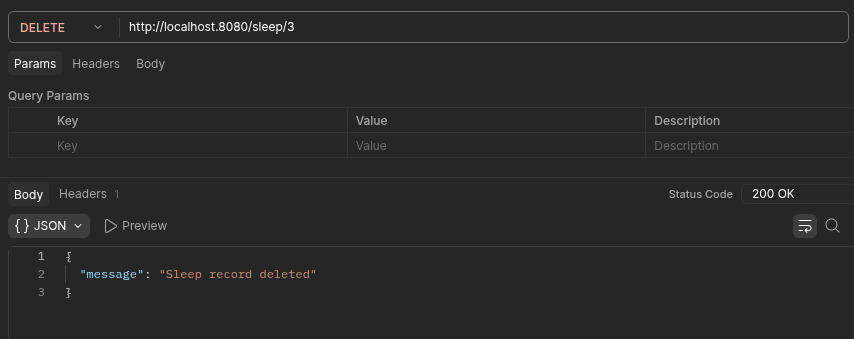
\includegraphics[width=1\textwidth]{images/postman/sleep_delete.png}
	\caption{Запрос удаления записи о сне}
	\label{fig:sleep_delete}
\end{figure}

\begin{figure}[H]
	\centering
	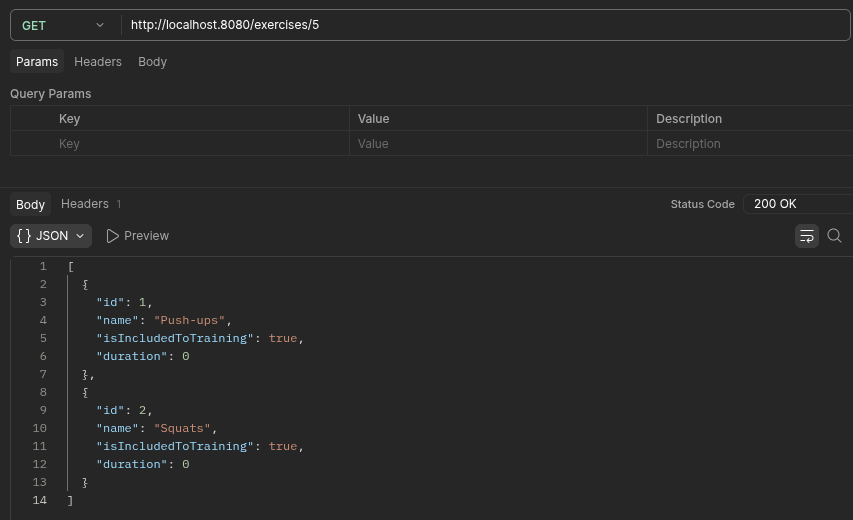
\includegraphics[width=1\textwidth]{images/postman/exercises_get.png}
	\caption{Запрос получения списка упражнений}
	\label{fig:exercises_get}
\end{figure}

\begin{figure}[H]
	\centering
	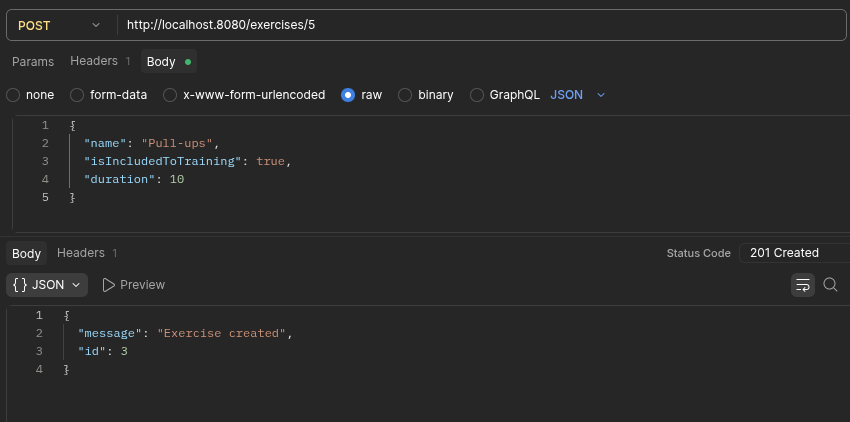
\includegraphics[width=1\textwidth]{images/postman/exercises_post.png}
	\caption{Запрос добавления упражнения}
	\label{fig:exercises_post}
\end{figure}

\begin{figure}[H]
	\centering
	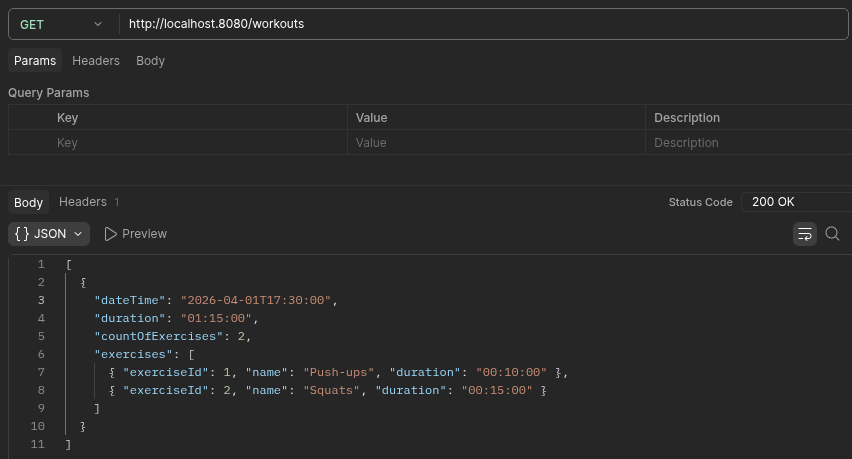
\includegraphics[width=1\textwidth]{images/postman/workouts_get.png}
	\caption{Запрос получения тренировок с упражнениями}
	\label{fig:workouts_get}
\end{figure}

\begin{figure}[H]
	\centering
	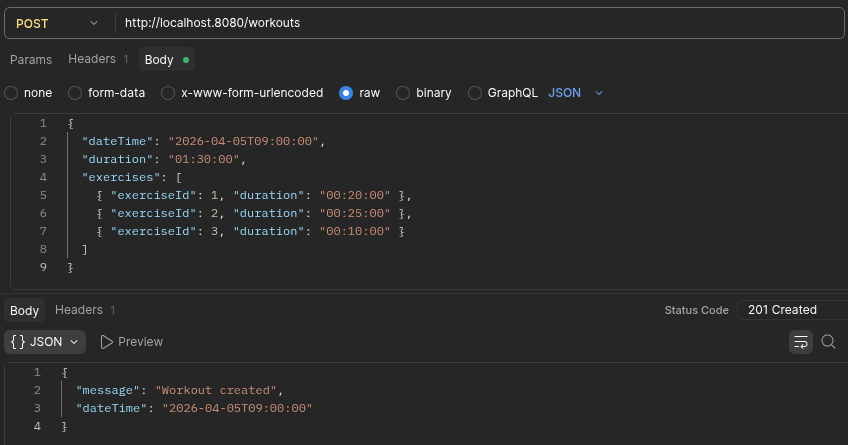
\includegraphics[width=1\textwidth]{images/postman/workouts_post.png}
	\caption{Запрос создания тренировки}
	\label{fig:workouts_post}
\end{figure}

\begin{figure}[H]
	\centering
	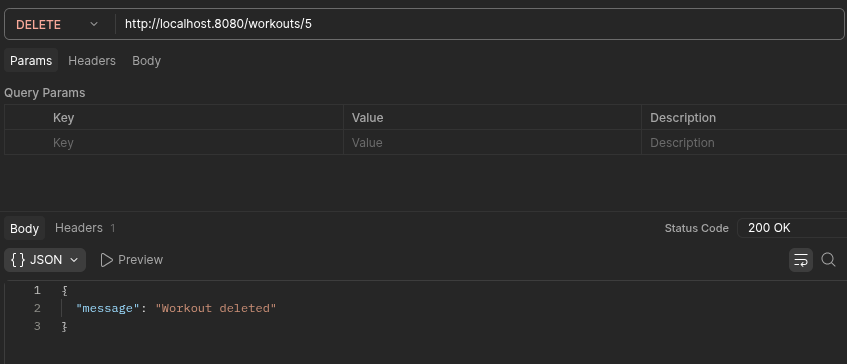
\includegraphics[width=1\textwidth]{images/postman/workouts_delete.png}
	\caption{Запрос удаления тренировки}
	\label{fig:workouts_delete}
\end{figure}

\nolabel{section}{Приложение 2}

\section*{Исходный код мобильного приложения и серверного приложения}


\begin{lstlisting}[caption={Структура многомодульного проекта}]
fit_app/
├── app/
├── presentation/
├── domain/
├── data/
└── di/
\end{lstlisting}

\begin{lstlisting}[caption={Доменные модели (domain)}]
// domain/model/Workout.kt
data class Workout(
    val id: String,
    val title: String,
    val description: String,
    val duration: Int,
    val exercises: List<Exercise>
)

data class Exercise(
    val id: String,
    val name: String,
    val duration: Int
)

data class SleepRecord(
    val id: String,
    val date: LocalDate,
    val durationMinutes: Int
)

data class History(
    val dateTime: LocalDateTime,
    val duration: Int,
    val exercisesCount: Int
)
\end{lstlisting}

\begin{lstlisting}[caption={Интерфейсы репозиториев (domain)}]
// domain/repository/LocalWorkoutRepository.kt
interface LocalWorkoutRepository {
    suspend fun getWorkouts(): List<Workout>
    suspend fun saveWorkout(workout: Workout)
}

// domain/repository/UserRemoteRepository.kt
interface UserRemoteRepository {
    suspend fun register(username: String, password: String, name: String): Result<UserData>
    suspend fun login(username: String, password: String): Result<Token>
}
\end{lstlisting}

\begin{lstlisting}[caption={Use case (доменная логика)}]
// domain/usecase/SleepRecommendationUseCase.kt
class SleepRecommendationUseCase(
    private val sleepRepo: LocalSleepRepository
) {
    suspend operator fun invoke(): String {
        val avg = sleepRepo.getAverageSleepForLastWeek()
        return when {
            avg < 6 -> "Для восстановления старайтесь спать 7–8 часов"
            avg < 7 -> "Постарайтесь увеличить сон на 30–60 минут"
            avg in 7..9 -> "Вы отлично высыпаетесь, поддерживайте режим"
            else -> "Возможна пересып, попробуйте сократить отдых"
        }
    }
}
\end{lstlisting}

\begin{lstlisting}[caption={ViewModel (presentation)}]
// presentation/ui/main/MainViewModel.kt
class MainViewModel(
    private val workoutRepo: LocalWorkoutRepository,
    private val sleepRepo: LocalSleepRepository,
    private val sleepRecommendation: SleepRecommendationUseCase
) : ViewModel() {

    private val _workouts = MutableStateFlow<List<Workout>>(emptyList())
    val workouts: StateFlow<List<Workout>> = _workouts

    private val _recommendation = MutableStateFlow("")
    val recommendation: StateFlow<String> = _recommendation

    init {
        viewModelScope.launch {
            _workouts.value = workoutRepo.getWorkouts()
            _recommendation.value = sleepRecommendation()
        }
    }
}
\end{lstlisting}

\begin{lstlisting}[caption={Compose экран (presentation)}]
// presentation/ui/main/MainScreen.kt
@Composable
fun MainScreen(viewModel: MainViewModel = koinViewModel()) {
    val workouts by viewModel.workouts.collectAsState()
    val recommendation by viewModel.recommendation.collectAsState()

    Scaffold(
        topBar = { TopAppBar(title = { Text("Фитнес-трекер") }) }
    ) { padding ->
        LazyColumn(modifier = Modifier.padding(padding)) {
            item {
                Card(colors = CardDefaults.cardColors(containerColor = Color.Yellow)) {
                    Text("Совет: $recommendation", modifier = Modifier.padding(16.dp))
                }
            }
            items(workouts) { workout ->
                WorkoutCard(workout) { /* навигация */ }
            }
        }
    }
}
\end{lstlisting}

\begin{lstlisting}[caption={Навигация (Jetpack Navigation)}]
// presentation/navigation/NavGraph.kt
@Composable
fun AppNavGraph(
    navController: NavHostController = rememberNavController(),
    startDestination: String = "auth"
) {
    NavHost(navController, startDestination) {
        composable("auth") { AuthScreen(navController) }
        composable("main") { MainScreen() }
        composable("training/{workoutId}") { backStackEntry ->
            val workoutId = backStackEntry.arguments?.getString("workoutId")!!
            TrainingScreen(workoutId)
        }
        composable("sleep_tracker") { SleepTrackerScreen() }
        composable("history") { HistoryScreen() }
        composable("profile") { ProfileScreen() }
    }
}
\end{lstlisting}

\begin{lstlisting}[caption={Room Entity и DAO (data)}]
// data/local/entity/WorkoutEntity.kt
@Entity(tableName = "workouts")
data class WorkoutEntity(
    @PrimaryKey val id: String,
    val title: String,
    val description: String,
    val duration: Int
)

// data/local/dao/WorkoutDao.kt
@Dao
interface WorkoutDao {
    @Query("SELECT * FROM workouts")
    suspend fun getAll(): List<WorkoutEntity>

    @Insert
    suspend fun insert(workout: WorkoutEntity)
}
\end{lstlisting}

\begin{lstlisting}[caption={Retrofit сервис и DTO (data/remote)}]
// data/remote/api/WorkoutApiService.kt
interface WorkoutApiService {
    @GET("workouts")
    suspend fun getWorkouts(): List<WorkoutDTO>

    @POST("workouts")
    suspend fun postWorkout(@Body workout: WorkoutDTO): WorkoutDTO
}

// data/remote/dto/WorkoutDTO.kt
data class WorkoutDTO(
    val id: String,
    val title: String,
    val duration: Int,
    val exerciseIds: List<String>
)
\end{lstlisting}

\begin{lstlisting}[caption={Реализация удалённого репозитория (data)}]
// data/repository/remote/WorkoutRemoteRepositoryImpl.kt
class WorkoutRemoteRepositoryImpl(
    private val api: WorkoutApiService,
    private val connectivityManager: ConnectivityManager
) : WorkoutRemoteRepository {

    override suspend fun getWorkouts(): Result<List<WorkoutDTO>> {
        return if (isNetworkAvailable()) {
            try {
                Result.success(api.getWorkouts())
            } catch (e: Exception) {
                Result.failure(e)
            }
        } else {
            Result.failure(NoInternetException())
        }
    }

    private fun isNetworkAvailable(): Boolean { ... }
}
\end{lstlisting}

\begin{lstlisting}[caption={Мапперы (data/mappers)}]
// data/mappers/WorkoutMapper.kt
fun WorkoutDTO.toDomain(exercises: List<Exercise>): Workout =
    Workout(
        id = id,
        title = title,
        description = "",
        duration = duration,
        exercises = exercises
    )

fun Workout.toDto(): WorkoutDTO =
    WorkoutDTO(
        id = id,
        title = title,
        duration = duration,
        exerciseIds = exercises.map { it.id }
    )
\end{lstlisting}

\begin{lstlisting}[caption={Внедрение зависимостей Koin (di)}]
// di/NetworkModule.kt
val networkModule = module {
    single { OkHttpClient.Builder().addInterceptor { chain ->
        val token = get<LocalUserRepository>().getToken()
        chain.proceed(chain.request().newBuilder().header("Authorization", "Bearer $token").build())
    }.build() }
    single { Retrofit.Builder().baseUrl("https://yourapi.com").client(get()).addConverterFactory(GsonConverterFactory.create()).build() }
    single { get<Retrofit>().create(WorkoutApiService::class.java) }
}

// di/RepositoryModule.kt
val repositoryModule = module {
    single<LocalWorkoutRepository> { LocalWorkoutRepositoryImpl(get(), get()) }
    single<WorkoutRemoteRepository> { WorkoutRemoteRepositoryImpl(get(), get()) }
}
\end{lstlisting}

\begin{lstlisting}[caption={Бэкенд: сущности Exposed}]
// entity/WorkoutEntity.kt
object Workouts : Table() {
    val id = varchar("id", 36).primaryKey()
    val userId = varchar("user_id", 36)
    val title = varchar("title", 100)
    val duration = integer("duration")
}
\end{lstlisting}

\begin{lstlisting}[caption={Бэкенд: DTO для API}]
// dto/WorkoutDTO.kt
@Serializable
data class WorkoutRequest(
    val title: String,
    val duration: Int,
    val exerciseIds: List<String>
)

@Serializable
data class WorkoutResponse(
    val id: String,
    val title: String,
    val duration: Int
)
\end{lstlisting}

\begin{lstlisting}[caption={Бэкенд: модуль Ktor с маршрутами (схема)}]
// Application.kt
fun Application.module() {
    install(CallLogging)
    install(ContentNegotiation) { json() }
    install(Authentication) {
        jwt {
            verifier(JwtVerifier)  // JwtVerifier не определён в этом фрагменте
            validate { credential ->
                if (credential.payload.getClaim("userId").asString() != null)
                    JWTPrincipal(credential.payload)
                else null
            }
        }
    }

    routing {
        post("/register") {
            val request = call.receive<RegisterRequest>()
            userRepository.register(request)      
            call.respond(HttpStatusCode.Created)
        }
        post("/login") {
            val request = call.receive<LoginRequest>()
            val token = authService.generateToken(request) // несуществующий сервис
            call.respond(TokenResponse(token))
        }
        authenticate {
            get("/workouts") {
                val userId = call.principal<JWTPrincipal>()!!.payload.getClaim("userId").asString()
                val workouts = workoutRepository.findByUser(userId) 
                call.respond(workouts)
            }
            post("/workouts") {
                val request = call.receive<WorkoutRequest>()
                workoutRepository.create(request)   
                call.respond(HttpStatusCode.Created)
            }
            delete("/workouts/{dateTime}") {
                val dateTime = call.parameters["dateTime"]!!
                workoutRepository.deleteByDateTime(dateTime) 
                call.respond(HttpStatusCode.NoContent)
            }
            get("/sleep") {
                val userId = call.principal<JWTPrincipal>()!!.payload.getClaim("userId").asString()
                val records = sleepRepository.findByUser(userId) 
                call.respond(records)
            }
            post("/sleep") {
                val request = call.receive<SleepRequest>()
                sleepRepository.add(request)        
                call.respond(HttpStatusCode.Created)
            }
            put("/sleep/{id}") {
                val id = call.parameters["id"]!!
                val request = call.receive<SleepRequest>()
                sleepRepository.update(id, request) 
                call.respond(HttpStatusCode.OK)
            }
            delete("/sleep/{id}") {
                val id = call.parameters["id"]!!
                sleepRepository.delete(id)           
                call.respond(HttpStatusCode.NoContent)
            }
        }
    }
}
\end{lstlisting}

\begin{lstlisting}[caption={Бэкенд: JWT генерация}]
// utils/Jwt.kt
fun generateToken(userId: String): String {
    return JWT.create()
        .withClaim("userId", userId)
        .withExpiresAt(Date(System.currentTimeMillis() + 86_400_000))
        .sign(Algorithm.HMAC256("secret"))
}
\end{lstlisting}

\begin{lstlisting}[caption={Бэкенд: подключение к PostgreSQL}]
// DatabaseFactory.kt
fun initDatabase() {
    Database.connect(
        "jdbc:postgresql://localhost:5432/fitdb",
        driver = "org.postgresql.Driver",
        user = "postgres",
        password = "123"
    )
    transaction {
        SchemaUtils.create(Users, Workouts, Exercises, SleepRecords)
    }
}
\end{lstlisting}